\documentclass[12pt]{scrartcl}

\usepackage[headsepline]{scrlayer-scrpage}
\usepackage[nenglish]{babel}
\usepackage{amssymb}
\usepackage{amsmath}
\usepackage{graphicx}


\title{SZ Solar Cell}
\author{Jonathan Witte, Matthias Gatter, Eduard Heidt\\ \\
	Tutor: Tao Wei\\ \\
	Protocol handed in: \\
	Version: 1}
\date{}
\pagestyle{scrheadings}

\begin{document}
	
	\pagenumbering{gobble}
	\maketitle
	\newpage
	
	
	\tableofcontents
	\newpage
	
	
	\automark{section}
	\pagenumbering{arabic}
	\ihead{SZ}
	\ohead{\pagemark}
	
	\newpage
	
	\section{Introduction}
	
	\section{Theory}
	
	\section{Experimental setup and procedure}
		To setup the experiment we take a lightsource, in our case a halogen lamp, a solar cell that we mount in front of the light source such that we can vary the distance. We connect a voltmeter and an amperemeter to measure the voltage between the two poles of the solar cell and the current that flows when we connect them. In series with the amperemeter we also connect a potentiometer to vary the resistance which will come in handy. Its schematics would look like this:
		
		\begin{figure}[h]
			\centering
			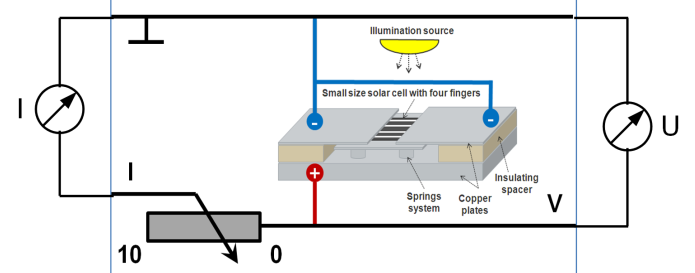
\includegraphics[width = 0.7 \linewidth]{Bilder/Schaltung.png}
			\label{Schaltung}
			\caption{schematic setup of the experiment}
		\end{figure}
	
		The procedure of the experiment is devided into some steps that are necessary for 
	\section{Evaluation}
	
\end{document}